\chapter{Data Samples}
\label{sec:DataSamples}

The data samples is the actual information about collisions recorded by the detector. This information is divided into periods, runs and luminosity blocks (LB). The luminosity block is the smallest of the three, its duration is decided by the ATLAS central trigger processor, and usually is one minute. The data taken within one LB is considered to have constant luminosity, which is calculated separately and stored in the luminosity database. To calculate the instantaneous luminosity, ATLAS uses several specialized detectors: the Minimum  Bias Trigger Scintillators (MBTS), which determines the start of the bunch crossing, the Beam Conditions Monitor (BCM) which was originally designed to monitor the beam losses and prevent the inner detector damage, but the data from which can be used to calculate luminosity, and the LUCID detector (LUminosity measurement using a Cherenkov Integrating Detector), which is specially designed to measure luminosity by the use of the Cherenkov radiation. The data from BCM and LUCID is captured during the data-taking, and is later scaled to the luminosity and beam conditions values provided by the LHC~\cite{lib:lumi}. The run represents the data taken during one continuous period of time. It can't be longer that one beam injection, but could be shorter, if some problems that lead to a halt in data taking were encountered during the injection. The period is a group of runs with the same detector conditions. Each period represents different setup of the detector and/or triggers and/or collider itself.

In 2011 there were 13 periods from A to M. Periods A and C were not physical runs, and the period B had only \ensuremath{16.98\,\mathrm{pb}^{-1}} worth of data while having the conditions substantially different from all the other runs and thus was excluded from the analysis.

During some of the runs there were discovered problems with the detector or with the triggers, which compromised the data. The LBs during which these problems occur should be excluded from the analysis, and it is done using the good run list (GRL) which lists all the runs and LBs which should be used. In this analysis the common GRL of the WZ group\\
(\texttt{\footnotesize data11\_7TeV.periodAllYear\_DetStatus-v36-pro10\_CoolRunQuery-00-04-08\_WZjets\_allchannels\_DtoM.xml})\\
is used.

The amount of data collected from the detector can be measured by it's integrated luminosity. In Section~\ref{sec:LHC} a definition of the instantaneous luminosity is given, which represents the amount of delivered data per unit of time. By integrating the instantaneous luminosity over data-taking time we can calculate the total amount of data delivered by LHC. When referring the luminosity without indication of whether it is instantaneous or integrated, it usually mean that the integrated luminosity is implied. The data taking process is also not absolutely effective, there are losses from trigger failures, DAQ system overloads, and just errors that prevented data taking at some period of time. The process of translating of the recorded luminosity to the delivered luminosity is thus not trivial, but can be done automatically by the use of the special tool~\footnote{Can be found here \url{https://atlas-lumicalc.cern.ch/}}, so in all the calculations only the delivered luminosity is used.

The total luminosity for full data set used in the analysis was calculated by summing the luminosity from all LBs and equals to \ensuremath{4.58\,\mathrm{fb}^{-1}} with the systematic uncertainty $1.8\%$~\cite{lib:lumi}. The timeline of data collection can be seen on Figure~\ref{fig:data}. The list of all periods with corresponding run numbers, integrated luminosity, maximum instantaneous luminosity and the default single electron trigger (which is the trigger used for the \Zee\ central forward analysis) is shown in Tab.~\ref{tab:data}. The triggers for the analysis were chosen because they were the lowest unprescaled single electron triggers for the corresponding periods. The process of prescaling is done for the low-energy triggers, because we have no resources to record all the events that match these triggers, so we record only the known fraction of them, e.g. one out of three. For the analysis to remain unbiased, the use of the unprescaled trigger is important. The single-electron trigger was used because of the detector geometry and the trigger system set-up: the trigger is only working in the central part of the detector, so while the central-central analysis uses the di-electron trigger, because both of the electrons is expected to be in the central area, the central-forward analysis has to use the single-electron one.

\begin{figure}
\center{
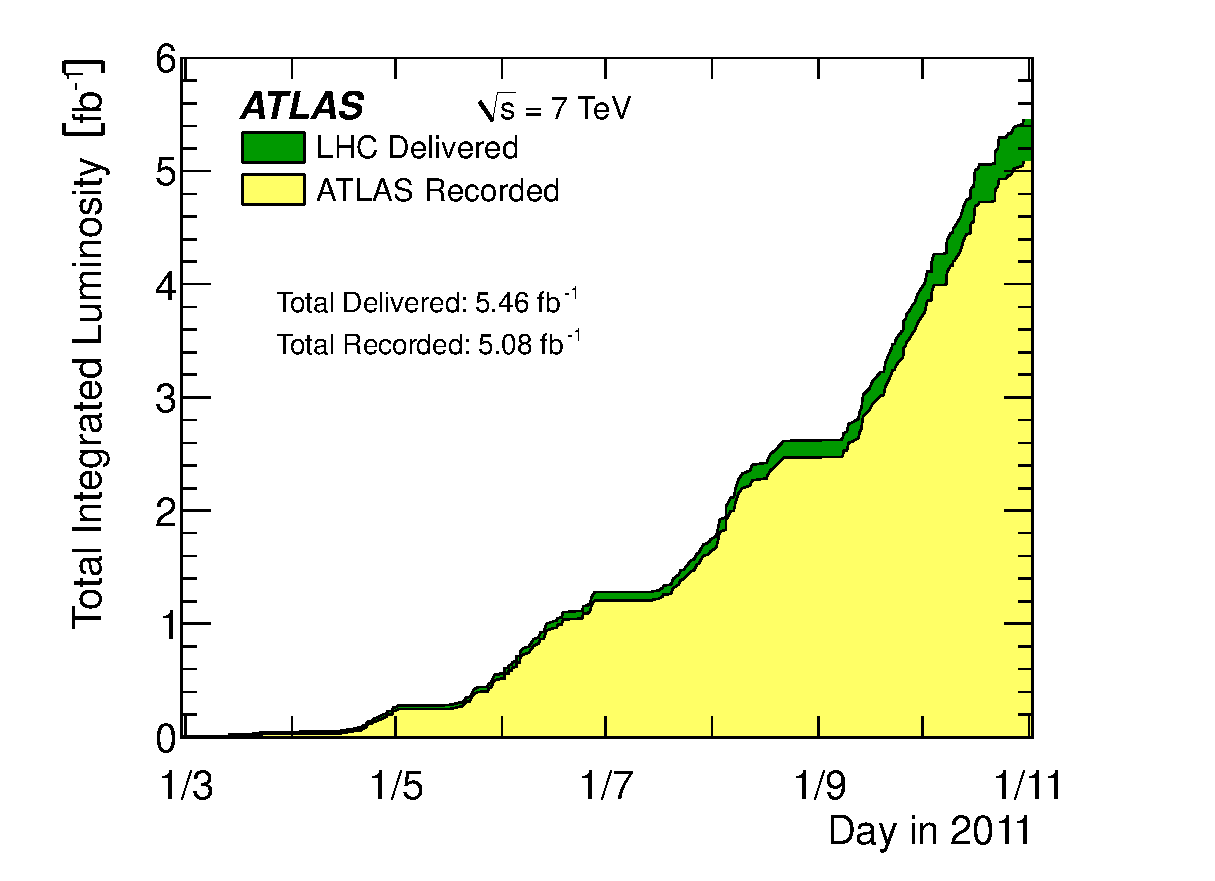
\includegraphics[width=1.0\textwidth]{figures/DATA_lumi.eps}
\caption{The integrated luminosity recorded by the ATLAS detector during 2011.}
\label{fig:data}}
\end{figure}


\begin{table}
\centering
\begin{tabular}{ c | cccl } \hline\hline
Period & Run Range & Lumi [$\rm pb^{-1}$] & Max Lumi $\rm [cm^{-2}s^{-1}]$ & Default SE trigger \\ \hline
D & 179710-180481 & $178.816$ & $6.65\times10^{32}$ & EF\_e20\_medium \\
E & 180614-180776 & $50.176$  & $8.37\times10^{32}$ & EF\_e20\_medium \\
F & 182013-182519 & $152.187$ & $1.11\times10^{33}$ & EF\_e20\_medium \\
G & 182726-183462 & $560.837$ & $1.27\times10^{33}$ & EF\_e20\_medium \\
H & 183544-184169 & $278.271$ & $1.27\times10^{33}$ & EF\_e20\_medium \\
I & 185353-186493 & $399.205$ & $1.90\times10^{33}$ & EF\_e20\_medium \\
J & 186516-186755 & $232.931$ & $2.02\times10^{33}$ & EF\_e20\_medium \\
K & 186873-187815 & $660.211$ & $2.35\times10^{33}$ & EF\_e22\_medium \\
L & 188902-190343 & $1568.848$ & $3.28\times10^{33}$ & EF\_e22vh\_medium1 \\
M & 190503-191933 & $1121.768$ & $3.61\times10^{33}$ & EF\_e22vh\_medium1 \\
\hline \hline
\end{tabular}
\caption{The list of 2011 ATLAS data periods used in the Z analysis.}
\label{tab:data}
\end{table}
